\chapter{Méthodologie}
\label{chap:4}

Dans les chapitres précédents, les différentes architectures d'habitats intelligents ainsi que les efforts mis en place pour y intégrer les \textit{wearable devices} ont été étudiés. De plus, les technologies aussi bien matérielles que logicielles spécifiques à ces dispositifs qui permettent de réaliser le processus d'apprentissage ont été détaillées et les problématiques qui y sont rattachées ont été exposées. 

Ainsi, ce projet propose, dans un premier temps, de développer de nouveaux types de \textit{wearable devices} dans l'optique d'améliorer l'assistance déjà offerte par les habitats intelligents. En effet, il semble que les technologies de reconnaissance existantes puissent être améliorées par de nouveaux systèmes faisant intervenir des \textit{wearable devices} qui agiraient alors en tant que solutions complémentaires. Dans un second temps, l'objectif de ce projet est de proposer un outil capable d'uniformiser les précédents travaux qui concernent l'assistance au sein des habitats intelligents avec des \textit{wearable devices}. En effet, grâce aux chapitres précédents, il est apparu que chaque solution existante impliquant ce type de dispositifs admet un fonctionnement entièrement autonome, c'est-à-dire mal intégré à l'environnement dans lequel il est utilisé (les habitats intelligents). De plus, pour réaliser le processus d'apprentissage, bien que la majorité des travaux incluent des composantes logicielles identiques, les données qui y sont exploitées n'appartiennent à aucune standardisation. Ainsi, l'idée est de proposer un outil simple à intégrer au sein d'un habitat intelligent et qui offrira la possibilité à tous les \textit{wearable devices} de fonctionner ensemble, mais également en combinaison avec les technologies \og statiques \fg de l'habitat.  

Ce quatrième et dernier chapitre va commencer par présenter l'infrastructure qui servira de base pour mener à bien ce projet de recherche qui s'articule en deux phases principales, chacune répondant aux différentes lacunes qui ont pu être observées dans les chapitres précédents. 

\section{Infrastructure : le \acs{LIARA}}

Ce projet de recherche va être réalisé grâce aux infrastructures offertes au \acs{LIARA}. Situé au sein de l'\ac{UQAC}, ce laboratoire offre un habitat intelligent complet d’une surface de cent mètres carrés dans lequel un grand volume de capteurs et d'effecteurs ambiant de types totalement différents y ont été intégrés. Le \acs{LIARA} est montré en figure \ref{fig:liara} En effet, il est question ici d’une centaine de capteurs tels que des contacteurs électromagnétiques, des thermomètres, des antennes et tags \acs{RFID}, des capteurs de luminosité, de débit d’eau et même de consommation électrique. De plus, le laboratoire offre également des effecteurs tels que des lumières contrôlées, des écrans et un système de haut-parleurs IP. L’intégralité de ces capteurs et effecteurs est connectée à une même base de données pour faciliter l’accès aux données et l’interaction avec l’infrastructure. Par exemple, des tapis de pression situés respectivement devant le lit et devant le lavabo de la salle de bain permettent de déterminer la présence d'une personne. De plus, des contacteurs électromagnétiques sont placés sur les placards et portes pour surveiller leurs ouvertures et fermetures. Enfin, les huit antennes \acs{RFID} permettent d'évaluer la position des objets qui sont équipés de tags et leur position est indiquée sur un écran qui affiche un plan du laboratoire.

\begin{figure}[H]
	\centering
	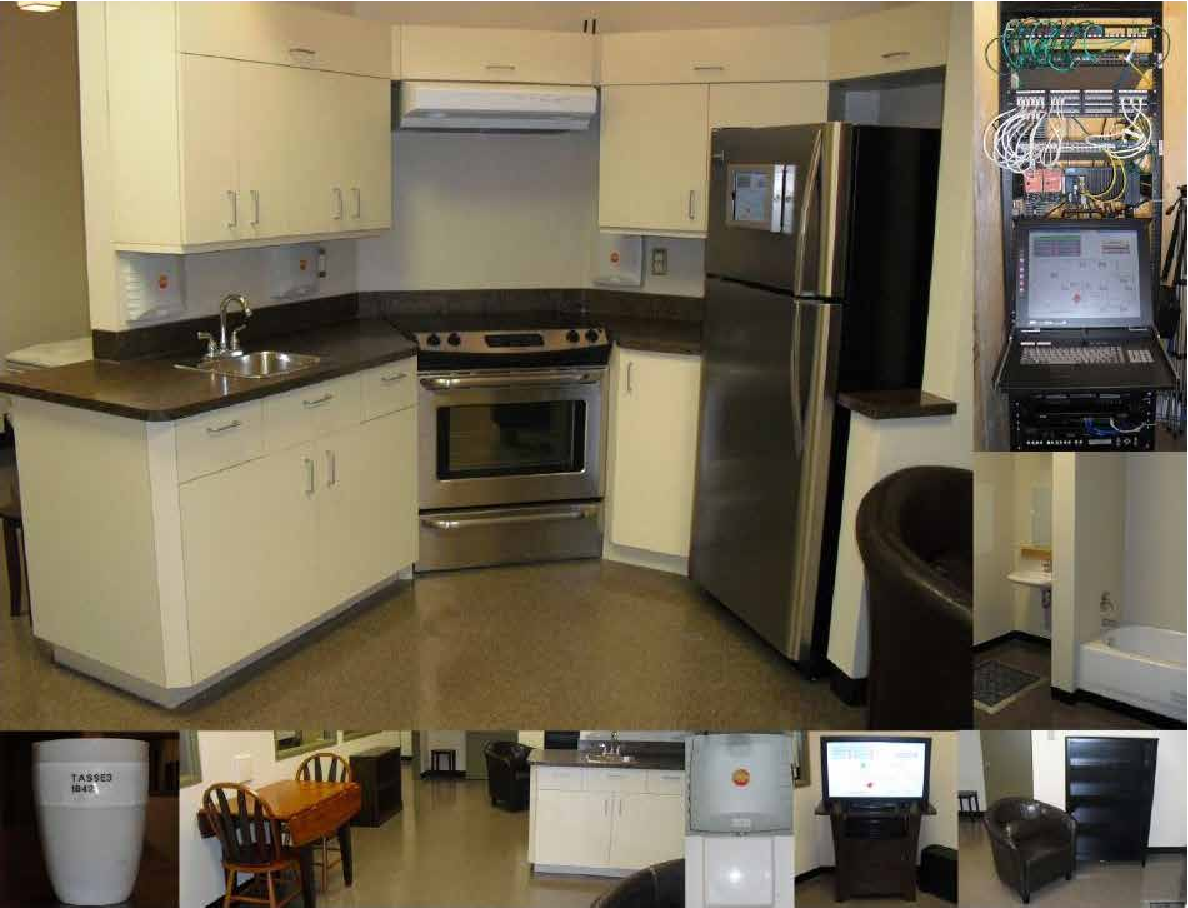
\includegraphics[width=.9\textwidth]{liara.pdf}
        \caption{Ensemble des pièces qui compose le \acs{LIARA}.}
	\label{fig:liara}
\end{figure}

Cette infrastructure constituera donc le cadre principal de toutes les expérimentations qui seront requises pour valider chacune des deux phases principales qui composent ce projet de recherche. 

\section{Phase I : avancements dans l'exploitation des \textit{wearable devices}}

Dans un premier temps, pour répondre à la première question énoncée en section \ref{sec:def_proj}, ce projet de recherche propose de s'intéresser à la conception de nouveaux \textit{wearable devices}. Ces derniers ont souvent été utilisés dans de nombreux domaines tels que la reconnaissance de gestes et d'activités, la réhabilitation ainsi que pour la surveillance de la santé au sein des habitats intelligents \citep{Khan2016, Davis2016, Chapron2018}. Cependant, certaines pistes qui permettraient d'améliorer l'assistance des résidents d'habitats intelligents semblent actuellement encore inexplorées. 

En ce sens, le premier \textit{wearable device} qui sera proposé dans ce projet de recherche va permettre de reconnaître les différents types de sols. Cette première contribution fera intervenir plusieurs algorithmes et technologies qui ont été présentés dans les chapitres précédents. En effet, une telle reconnaissance sera réalisée sur des données inertielles générées par le dispositif qui sera porté à différents endroits par un utilisateur. Cette idée est principalement issue du domaine de la robotique, où plusieurs travaux ont proposé cette idée pour améliorer la démarche des robots \citep{Bibuli2007a, Weiss2007a, Kertesz2016a}. Plus récemment, cette idée a également été expérimentée par \cite{Otis2016a} qui ont proposé l'utilisation d'une chaussure embarquant un accéléromètre. Cette dernière, capable de reconnaître les différents types de sols sur lesquels ses utilisateurs marchaient, avait pour objectif principal de déterminer un niveau de risque de chute et, en cas de danger, prévenir les marcheurs par une vibration sous le pied. 

Les objectifs visés par cette première contribution s'intègrent parfaitement dans l'optique d'assistance au sein d'un habitat intelligent, car ceux-ci peuvent comporter différents types de sols qui peuvent constituer des dangers ou causer de la peur chez les résidents. Par exemple, il est possible de mentionner les tapis, le carrelage mouillé dans la salle de bain ou encore les marches. Par conséquent, il demeure assez simple de voir comment une telle reconnaissance pourrait être intégrée à un \textit{wearable device} existant plus complet, déjà utilisé pour l'assistance au sein d'un habitat intelligent. De plus, l'idée de reconnaître des types de sol grâce à un \textit{wearable device} pourrait être adaptée à d'autres domaines comme celui du sport où ces dispositifs sont très largement utilisés \citep{Nielsen2014b}.

La seconde contribution visant à faire avancer l'exploitation des \textit{wearable devices} au sein des habitats intelligents concerne la conception d'une carte intelligente pour la sécurité d'accès et la personnalisation de ces habitats. En effet, chaque habitant étant unique, il possède nécessairement des habitudes et des goûts qui lui sont propres, comme la température d'une pièce. Il convient donc de trouver un moyen d'adapter la maison intelligente, non seulement à la maladie de son habitant, mais aussi aux préférences de celui-ci. Pour ce faire, ce projet de recherche proposera un second dispositif capable d'utiliser la démarche, qui est une donnée biométrique reconnue, pour identifier son porteur. Grâce à la combinaison de la reconnaissance de la démarche ainsi qu'à un tag \acs{NFC} embarqué directement dans la carte, l'accès à l'habitat intelligent pourra être sécurisé efficacement. De plus, ce dispositif pourra, après cette première vérification, aviser l'environnement des préférences de son porteur.

\section{Phase II : interopérabilité des \textit{wearable devices} au sein des habitats intelligents}

Dans un second temps, ce projet va proposer un système permettant de mieux intégrer les \textit{wearable devices} dans les habitats intelligents. En effet, les différentes architectures qui ont été proposées pour la conception de ces habitats n’ont pas été initialement prévues pour accueillir ces dispositifs. Par conséquent, ceux-ci se retrouvent très mal, voir nullement intégrés au sein des habitats intelligents. 

Ainsi, pour répondre aux questions \ref{question:2} et \ref{question:3} de la définition de ce projet de thèse, cette seconde phase a pour but de concevoir un outil capable de gérer à la fois les capteurs ambiants d'un habitat intelligent et les \textit{wearable devices} qui y sont utilisés. Ceci permettra alors de mettre en place une reconnaissance basée sur la fusion de ces sources de données diverses. Cet outil adoptera une conception modulaire permettant d'y ajouter des fonctionnalités supplémentaires, par exemple, un nouvel algorithme d'apprentissage. Aussi, il offrira la possibilité de réutiliser les différentes techniques qui composent le processus de reconnaissance d'activités détaillées dans le chapitre \ref{chap:2}. De ce fait, et en considérant une utilisation dans un cadre académique, cela simplifiera le développement de futurs dispositifs ainsi que les procédures expérimentales. Enfin, pour vérifier l'apport quant à une meilleure intégration des \textit{wearable devices} au sein des habitats intelligents, l'outil proposé devra, au minimum, être facilement déployable dans le type d'architecture du \acs{LIARA}.

\section{Planification}

Cette section présente la planification prévisionnelle donnée sous forme de diagramme GANTT par la figure \ref{fig:planification} expose un estimé du temps nécessaire à la réalisation de chaque tâche pour atteindre les objectifs de ce projet de recherche. 

\begin{figure}[H]
    \begin{sideways}
     \begin{minipage}{.7\textheight}
        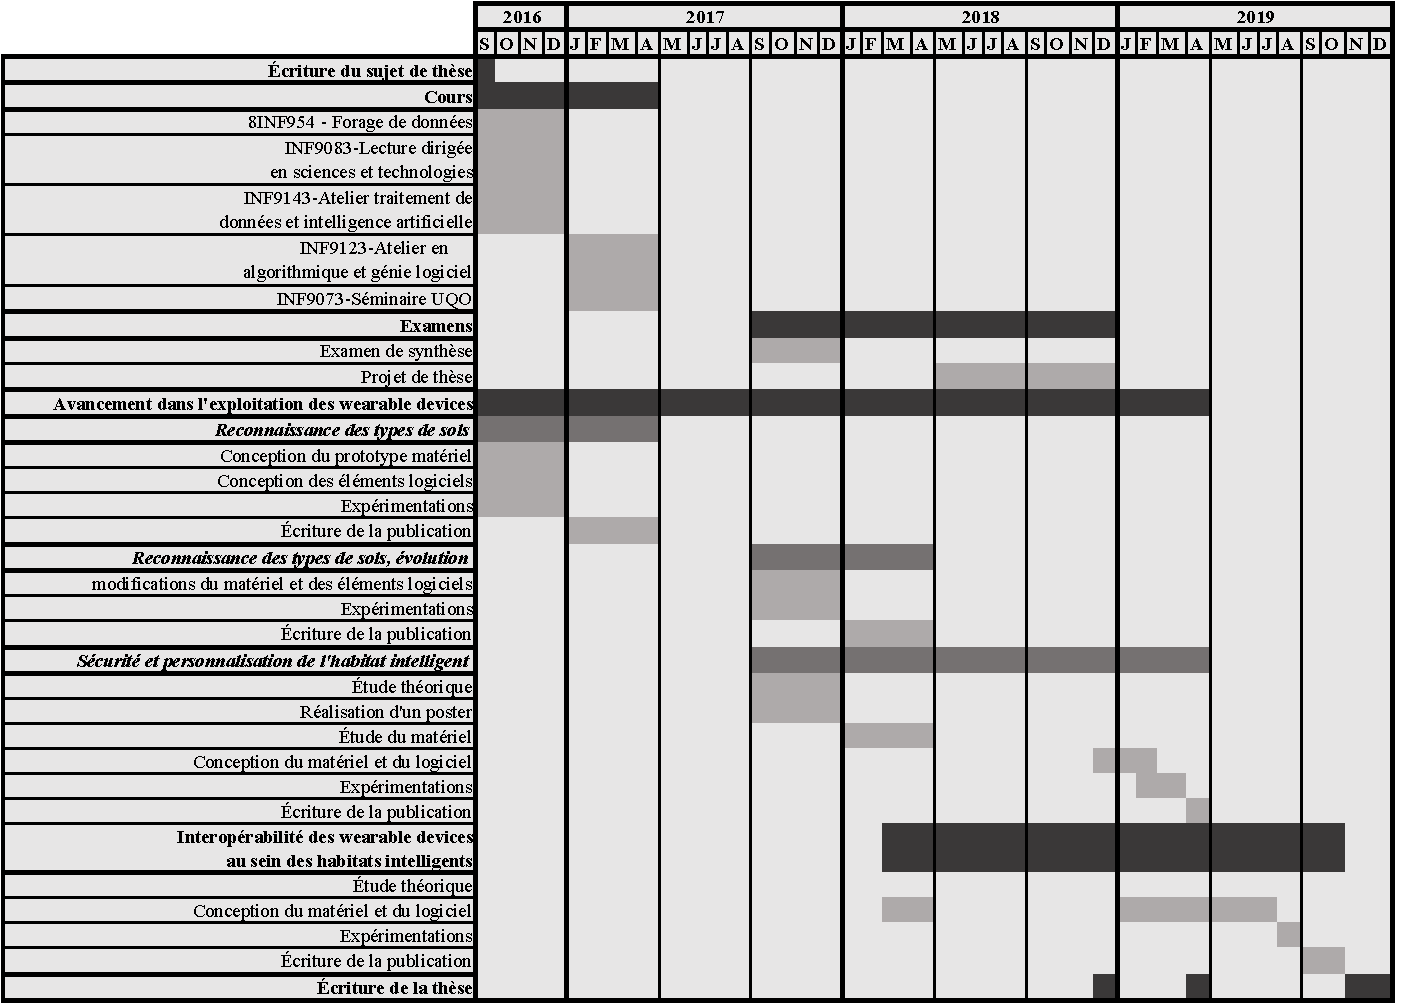
\includegraphics[width=\textwidth]{planification.pdf}
     \end{minipage}
    \end{sideways}
    \centering
    \caption{Planification de la thèse.}
    \label{fig:planification}
\end{figure}
